
\hypertarget{sensitivituxe4t-analysen-.rvp-datei}{%
\part{Sensitivität analysen (.rvp
Datei)}\label{sensitivituxe4t-analysen-.rvp-datei}}

\begin{frame}{Sensitivität Index}
\protect\hypertarget{sensitivituxe4t-index}{}
\[
SI_{NSE}=\frac{NSE_{max} - NSE_{33}}{1-NSE_{50}}
\]

\begin{itemize}
\item
  \(SI_{NSE}\): Sensitivität Index mit NSE
\item
  \(NSE_{max}\): Maximale (besten) NSE
\item
  \(NSE_{33}\), \(NSE_{55}\): 33\%, 55\% Quantile von NSE-REihe
\end{itemize}
\end{frame}

\begin{frame}{SoilParameter darstellen}
\protect\hypertarget{soilparameter-darstellen}{}
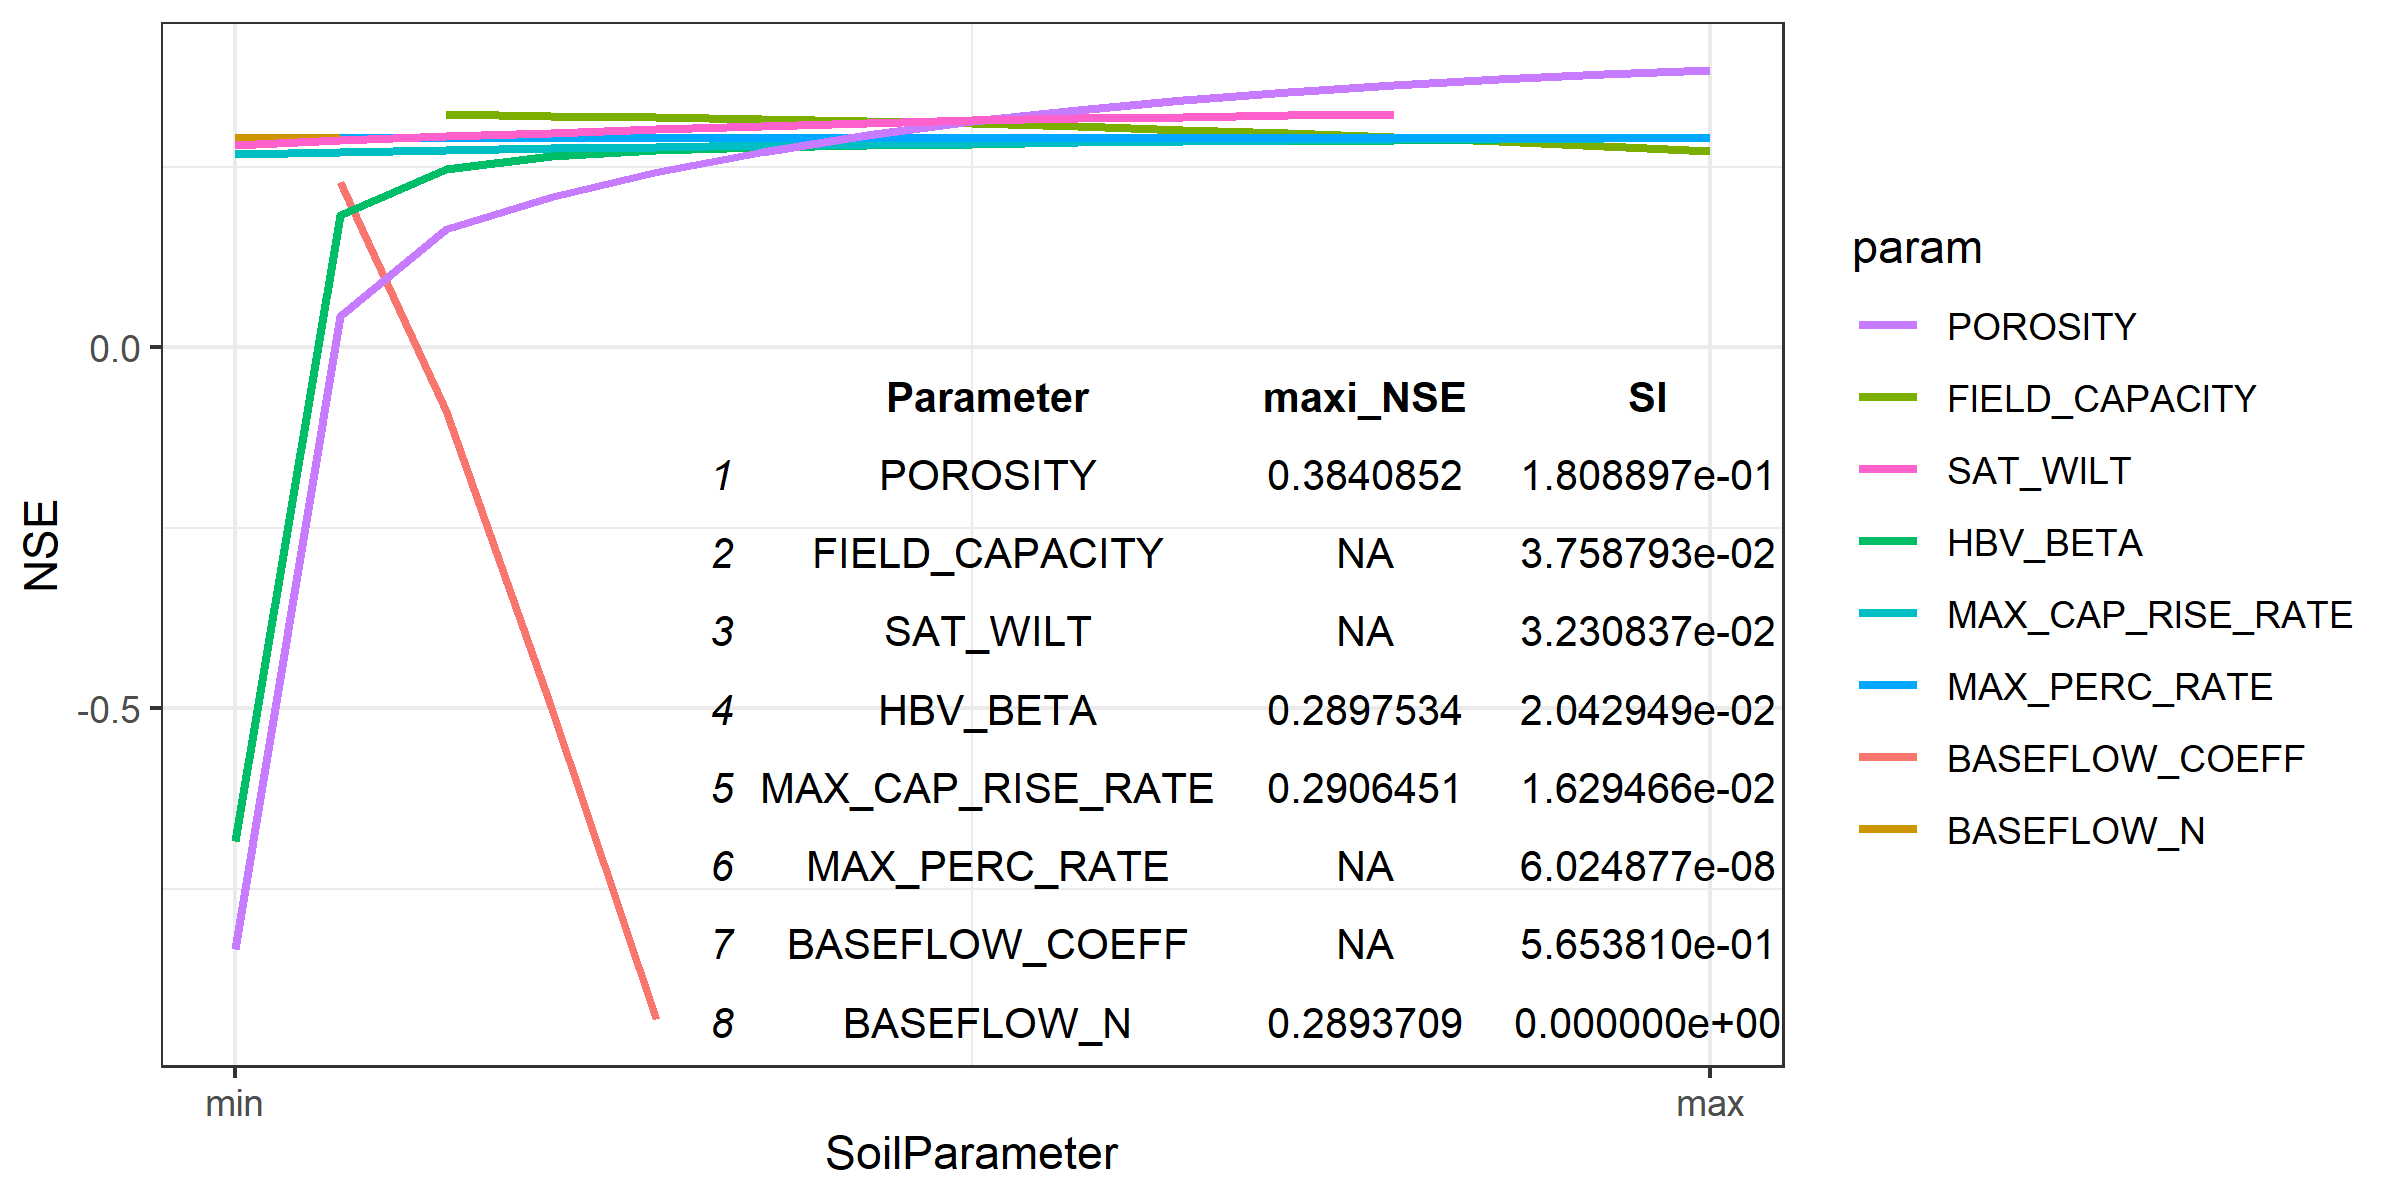
\includegraphics{plot_soil.png} \#\#\#\# VegetatioParameter darstellen

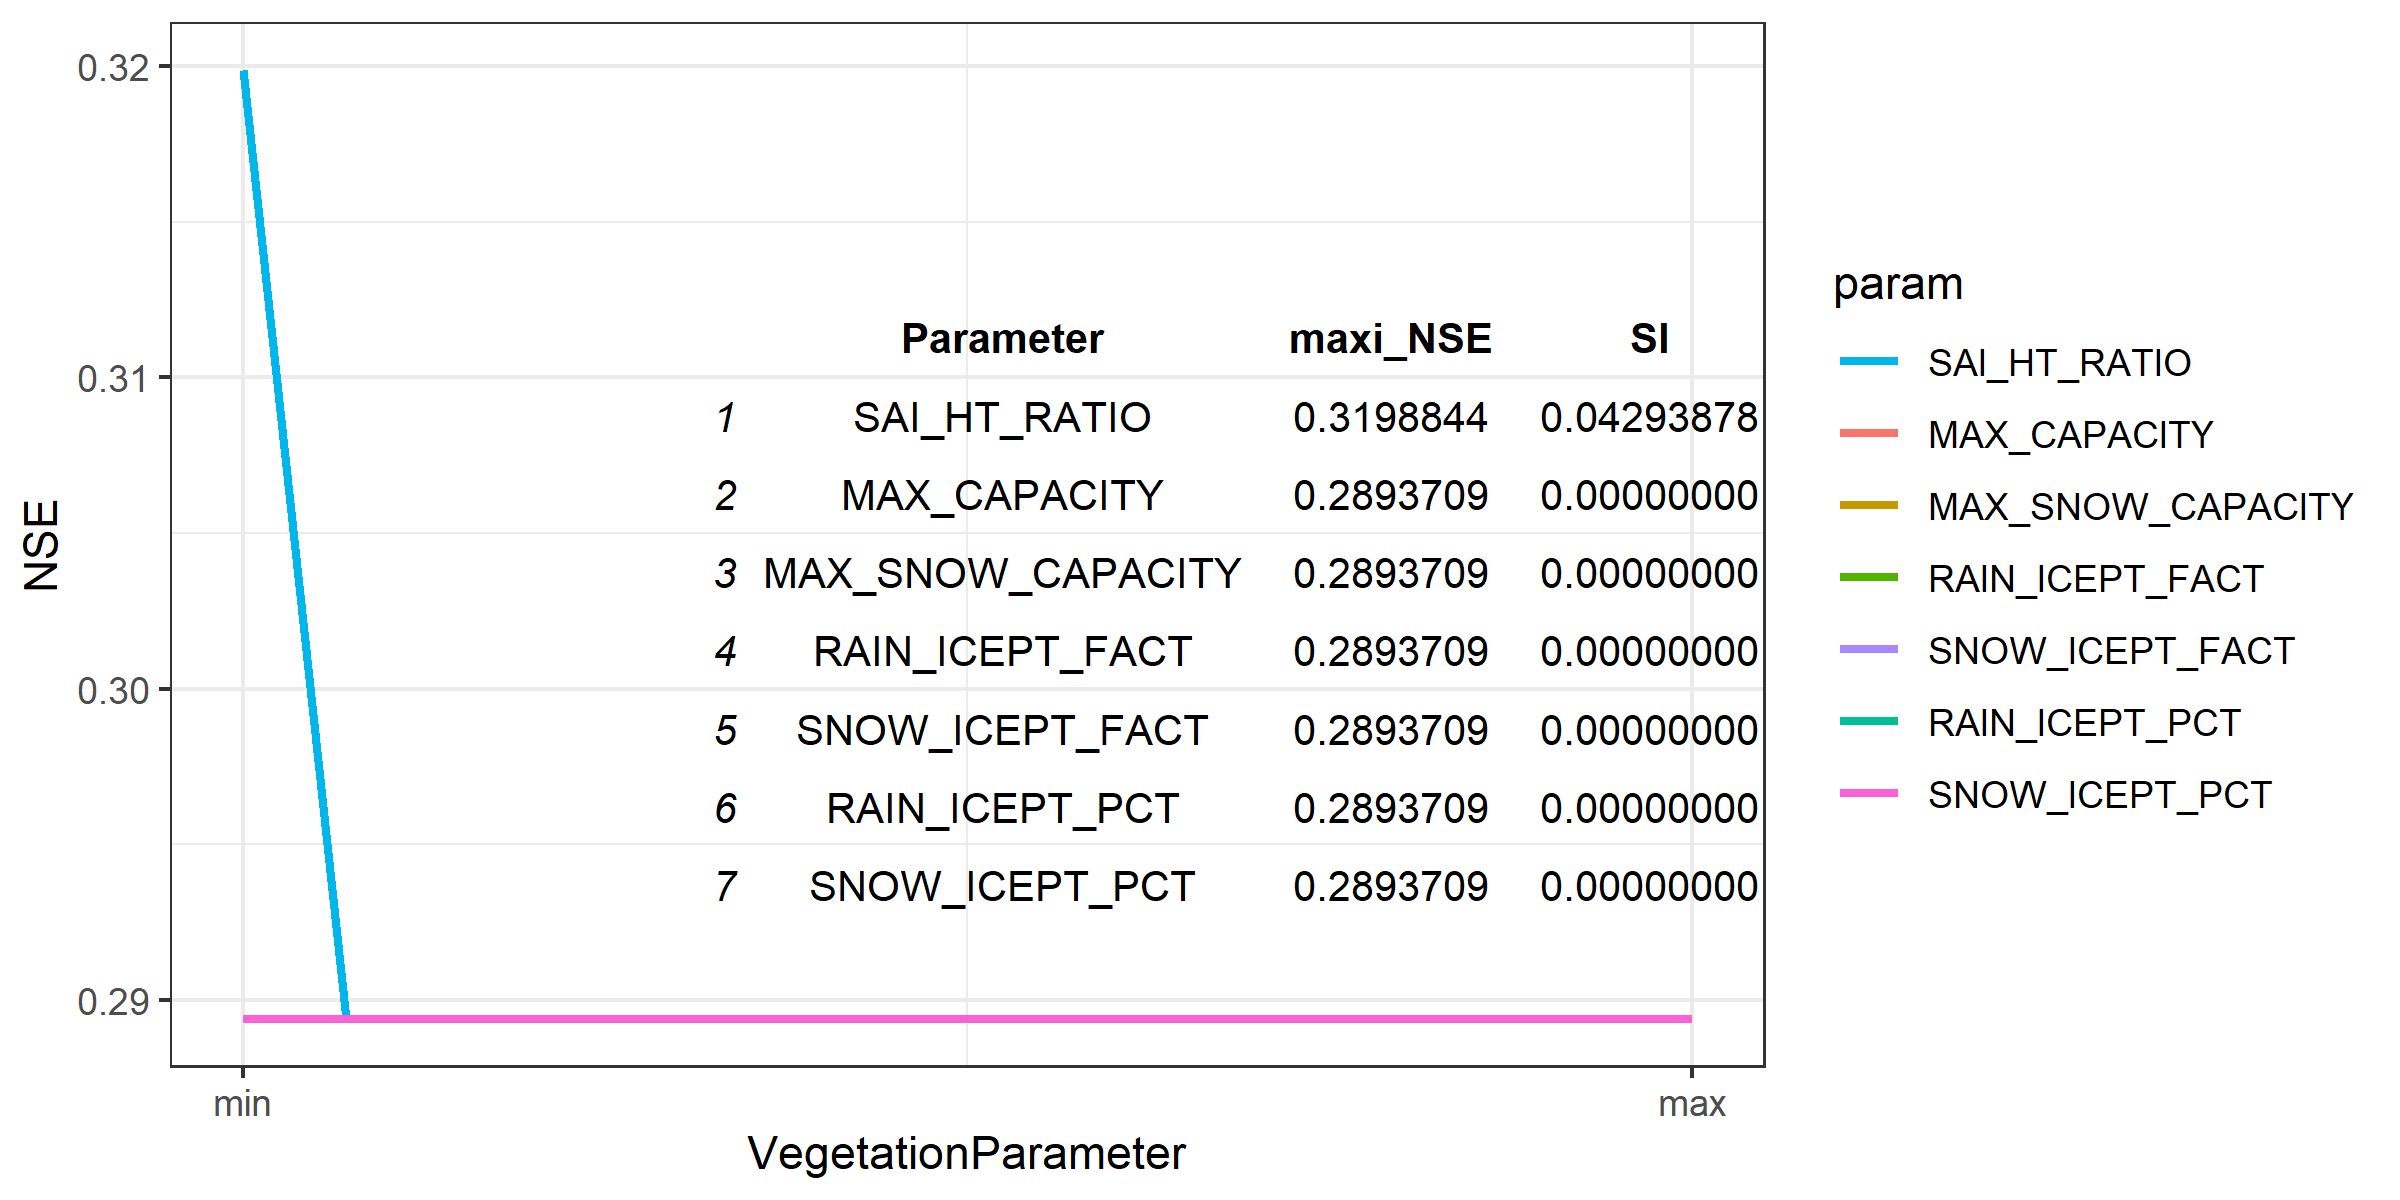
\includegraphics{plot_Veg.png}
\end{frame}

\begin{frame}{LanduseParameter darstellen}
\protect\hypertarget{landuseparameter-darstellen}{}
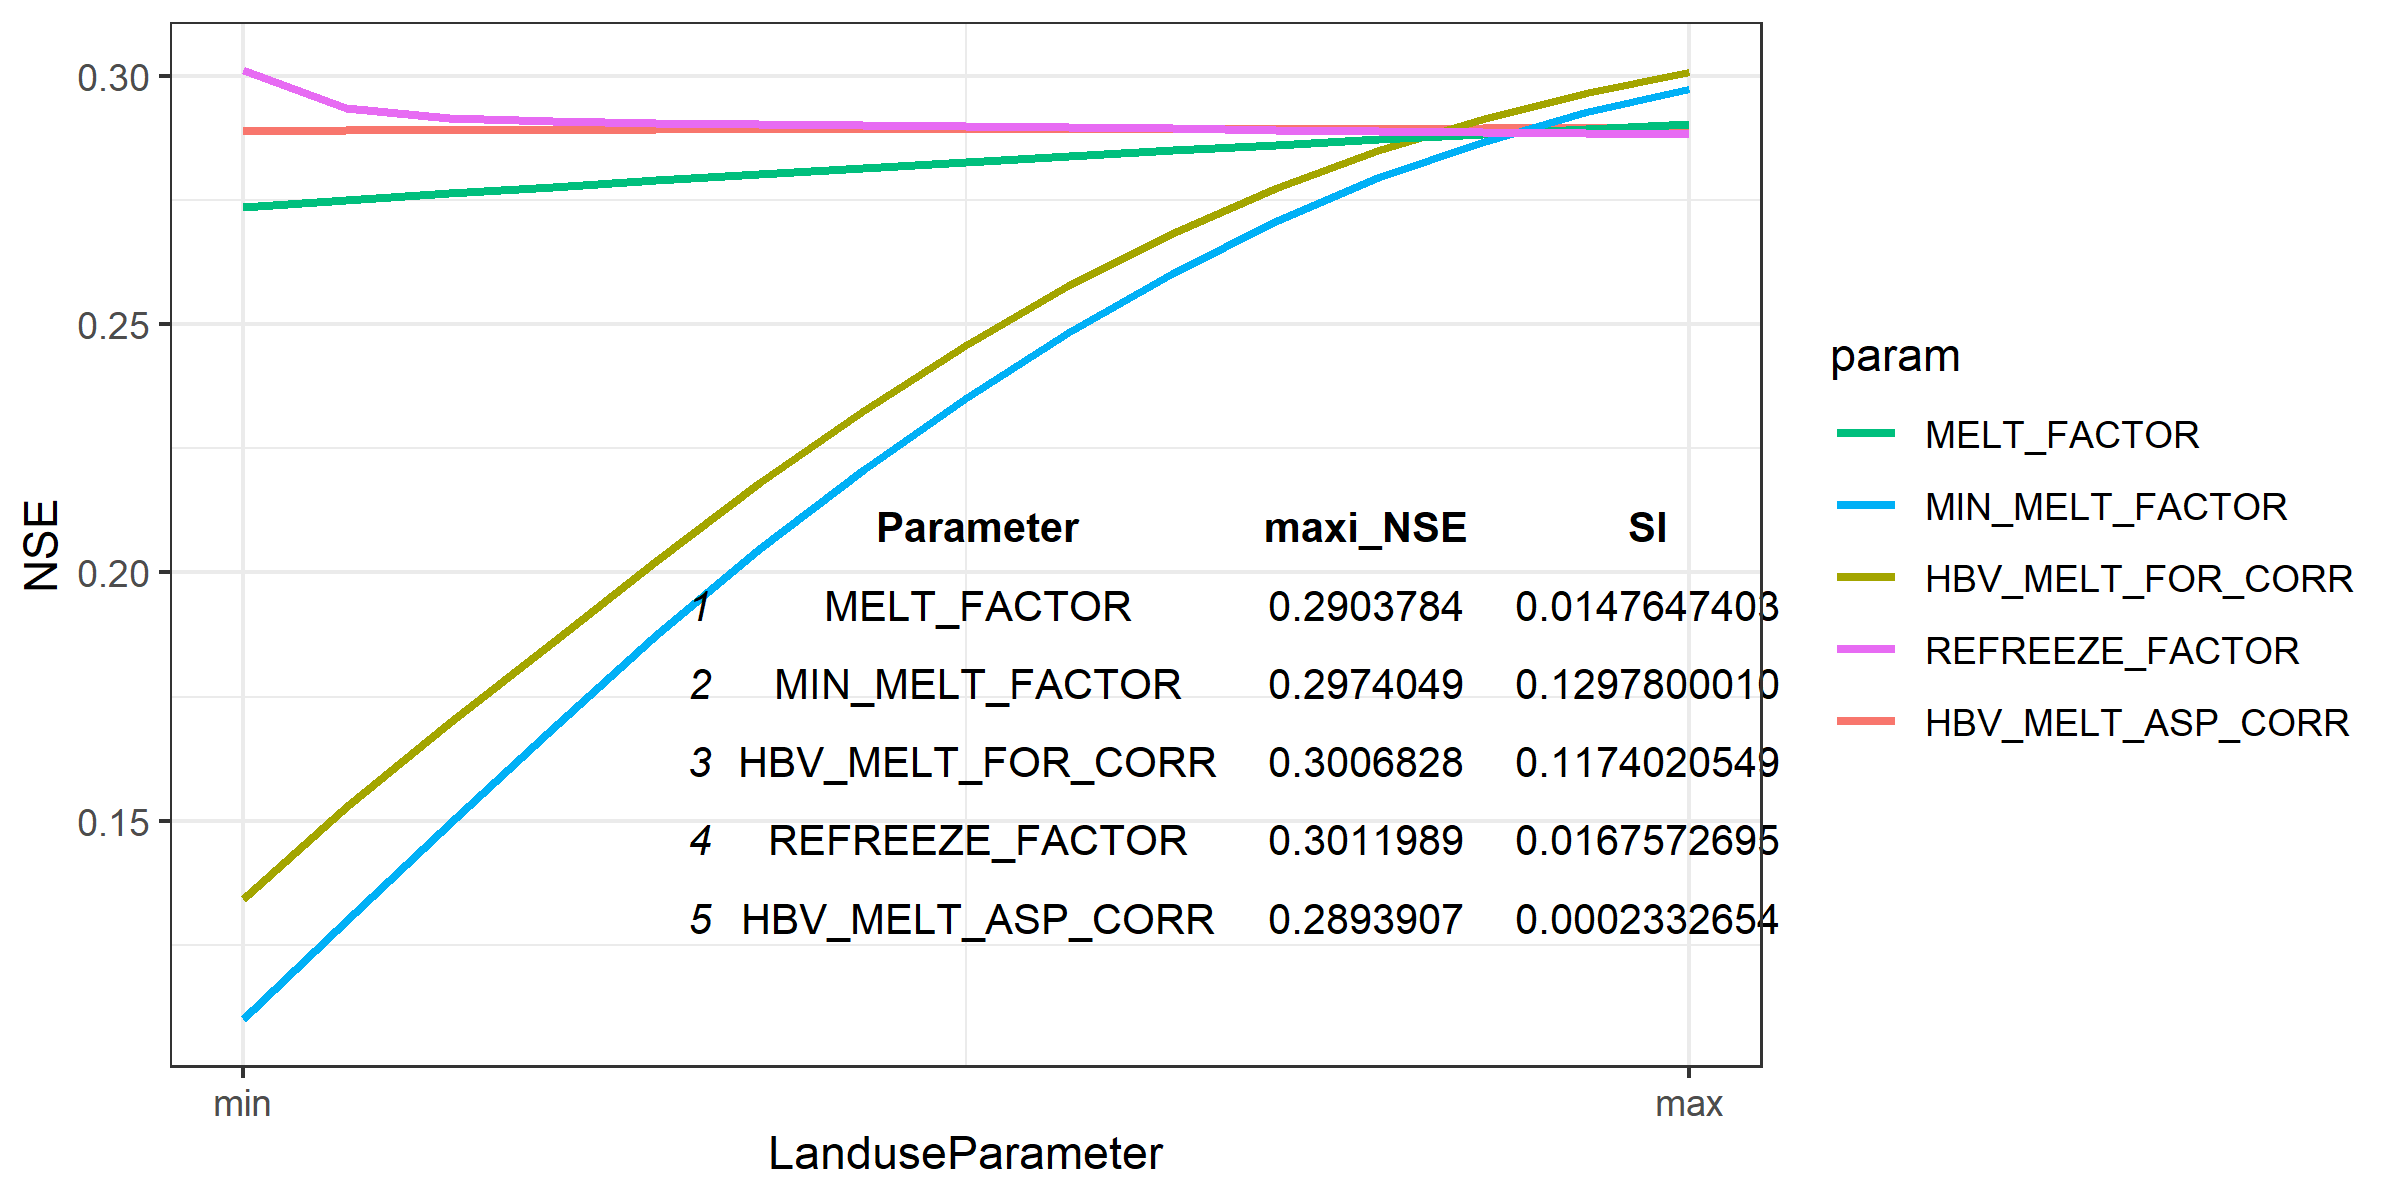
\includegraphics{plot_Land.png}
\end{frame}
